\documentclass[aspectratio=169]{beamer}
\setbeamertemplate{navigation symbols}{}
\usepackage{color,amsmath,comment, subfigure}
\usepackage{booktabs}
\def\vf{\vfill}
\usepackage{url}

%\setbeameroption{show notes}

%%%%%%%%%%%%%%%%%%%%%%%%%%
\title[]{Class 10: Thresholds, cascades, and predictability}
\author[]{Matthew J. Salganik}
\institute[]{Sociology 204: Social Networks\\Princeton University}
\date[]{
1/2 Threshold model
\vfill
\begin{flushleft}
\vspace{0.6in}

\includegraphics[width=0.1\textwidth]{figures/cc.png}
\end{flushleft}

}

%
%Movie suggested by former student
%\url{https://www.ted.com/talks/derek_sivers_how_to_start_a_movement#t-47105}

\begin{document}
%%%%%%%%%%%%%%%%%%%%%%%%%%%
\frame{\titlepage}
%%%%%%%%%%%%%%%%%%%%%%%%%%%
\begin{comment}
\begin{frame}

SWBAT:
\begin{enumerate}
\item diseases and social fad have different micro rule and macro dynamics
\item 
\end{enumerate}

\end{frame}
\end{comment}
%%%%%%%%%%%%%%%%%%%%%%%%
\begin{frame}

Summary:
\begin{itemize}
\item many decisions are interdependent
\pause
\item when there are interdependent decisions, individual rationality can lead to collective irrationality
\end{itemize}

\end{frame}
%%%%%%%%%%%%%%%%%%%%%%%%%
\begin{frame}

\begin{center}
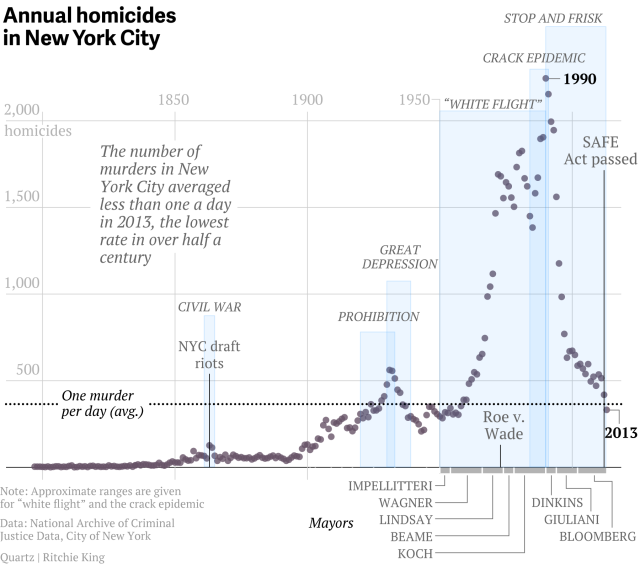
\includegraphics[width=0.6\textwidth]{figures/ny-murder-rates}
\end{center}

\tiny{\url{http://qz.com/162289/217-years-of-homicide-in-new-york/}}

\note{
Gladwell starts with NYC murder rates

note that he starts his time series is a specific place
}

\end{frame}
%%%%%%%%%%%%%%%%%%%%%%%%%
\begin{frame}

Nonlinear change

\begin{figure}
  \centering
     \subfigure{
     
\includegraphics[width=0.3\textwidth]{figures/Seinfeld_Ketchup}}
  \hspace{0in}
  \subfigure{
\onslide<2->{\includegraphics[width=0.3\textwidth]{figures_book/2_2}}}
  \hspace{0in}
  \subfigure{
\onslide<3->{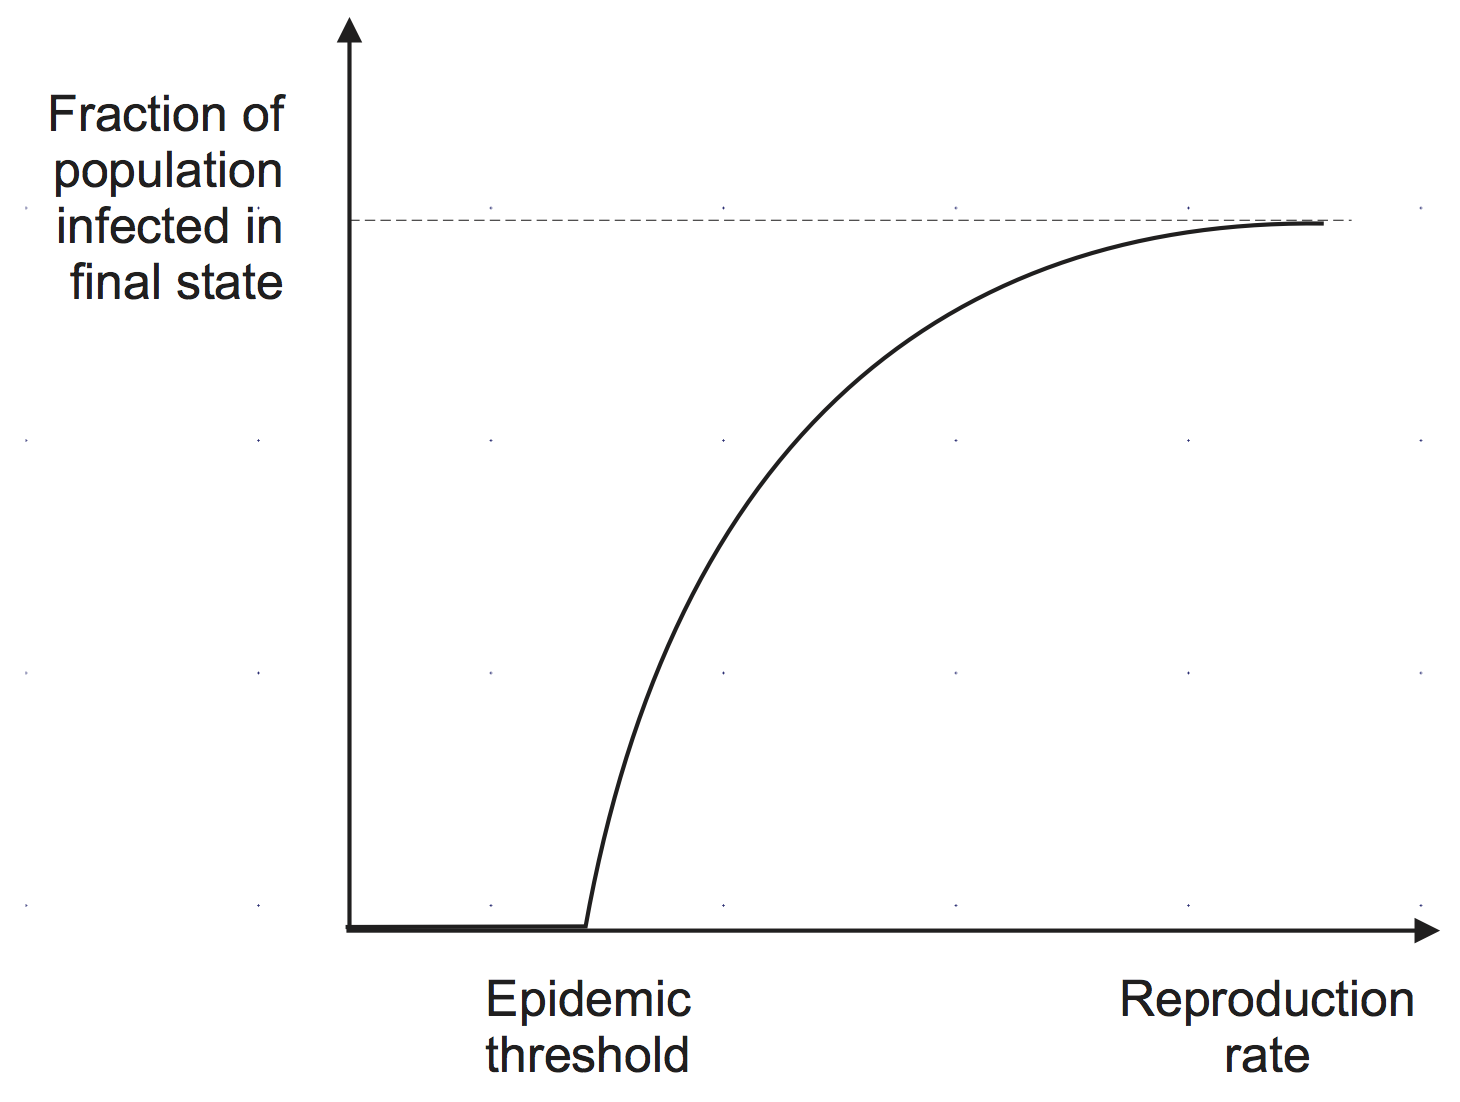
\includegraphics[width=0.3\textwidth]{figures_book/6_5_tight}}}
\end{figure}

\vf
\tiny{\url{http://www.davidmelamed.com/2013/07/15/user-testing-ketchup-bottles-leads-to-counter-intuitive-surge-in-profits/}}

\note{

When reading Gladwell's description of the flu in Manhattan you should have recognized $R_0$.

}

\end{frame}
%%%%%%%%%%%%%%%%%%%%%%%%%%
\begin{frame}

``What if homicides, which we often causally refer to as an epidemic, actually \emph{is} an epidemic, and moves through the populations the way that the flu bug does.''
Malcolm Gladwell

\end{frame}
%%%%%%%%%%%%%%%%%%%%%%%%%%
\begin{frame}

\setcounter{subfigure}{0}% Reset subfigure counter
\begin{figure}
  \centering
     \subfigure[Probability of activation in disease spreading]{
     \includegraphics[width=0.45\textwidth]{figures_book/8_1}}
  \hspace{0in}
  \subfigure[Probability of activation in social spreading]{
     \includegraphics[width=0.45\textwidth]{figures_book/8_2}}
\end{figure}

\vfill
\tiny{
For more on why social decisions might involve thresholds, see Lopez-Pintado and Watts (2008) \href{http://dx.doi.org/10.1177/1043463108096787}{\textcolor{blue}{Social Influence, Binary Decisions and Collective Dynamics}}}

\note{
Be skeptical of discontinuous change

There are many different models of decision making that bring about a threshold for social things.  Cost-Benefit is an easy one to understand

}

\end{frame}
%%%%%%%%%%%%%%%%%%%%%%%%%%
\begin{frame}

Differences between models of social contagion and biological contagion:
\begin{itemize}
\item social contacts are interdependent and disease contacts are independent
\pause
\item social spreading on fraction of neighbors doing some behavior rather than absolute number: diseases depends on absolute number
\end{itemize}

\end{frame}
%%%%%%%%%%%%%%%%%%%%%%%%%%
\begin{frame}

\begin{center}
\includegraphics[width=0.8\textwidth]{figures_book/8_2}
\end{center}

\end{frame}
%%%%%%%%%%%%%%%%%%%%%%%%%%
\begin{frame}

Standing ovation demo (imagine 100 students in a classroom)\\
\pause
Person 1, 0\\
Person 2, 1/100\\
Person 3, 2/100\\
Person 4, 3/100\\
Person 5, 4/100\\
$\ldots$
\note{

In person, bring up two groups of 10 students.  Each person gets a threshold written on an index card.  Two groups have different behavior.  Then, have everyone write their threshold on board.  Then we can see that the distributions are very similar.

Big difference in outcome
}

\end{frame}
%%%%%%%%%%%%%%%%%%%%%%%%%%%
\begin{frame}

Standing ovation demo (imagine 100 students in a classroom)\\
\pause
Person 1, 0\\
Person 2, 2/100\\
Person 3, 2/100\\
Person 4, 3/100\\
Person 5, 4/100\\
$\ldots$
\note{

Assume that there are 100 people in the room.

Assign Andres threshold 0, Andrew threshold 0.01, next person 0.02, 0.03, 0.04, 0.05, etc

Play out dynamics

Next assign 0, 0.02, 0.02, 0.03, 0.04, etc

Big difference in outcome

}

\end{frame}
%%%%%%%%%%%%%%%%%%%%%%%%%%%
\begin{frame}

Demo illustrates that 
\begin{itemize}
\item hard to predict collective outcome from individual preferences
\pause
\item hard to infer individual preferences from collective outcomes
\end{itemize}

\vfill
\tiny{For more examples, see Granovetter (1978) \href{http://www.jstor.org/stable/2778111}{\textcolor{blue}{Threshold Models of Collective Behavior}}}

\end{frame}
%%%%%%%%%%%%%%%%%%%%%%%%%%%
\begin{frame}

\begin{center}
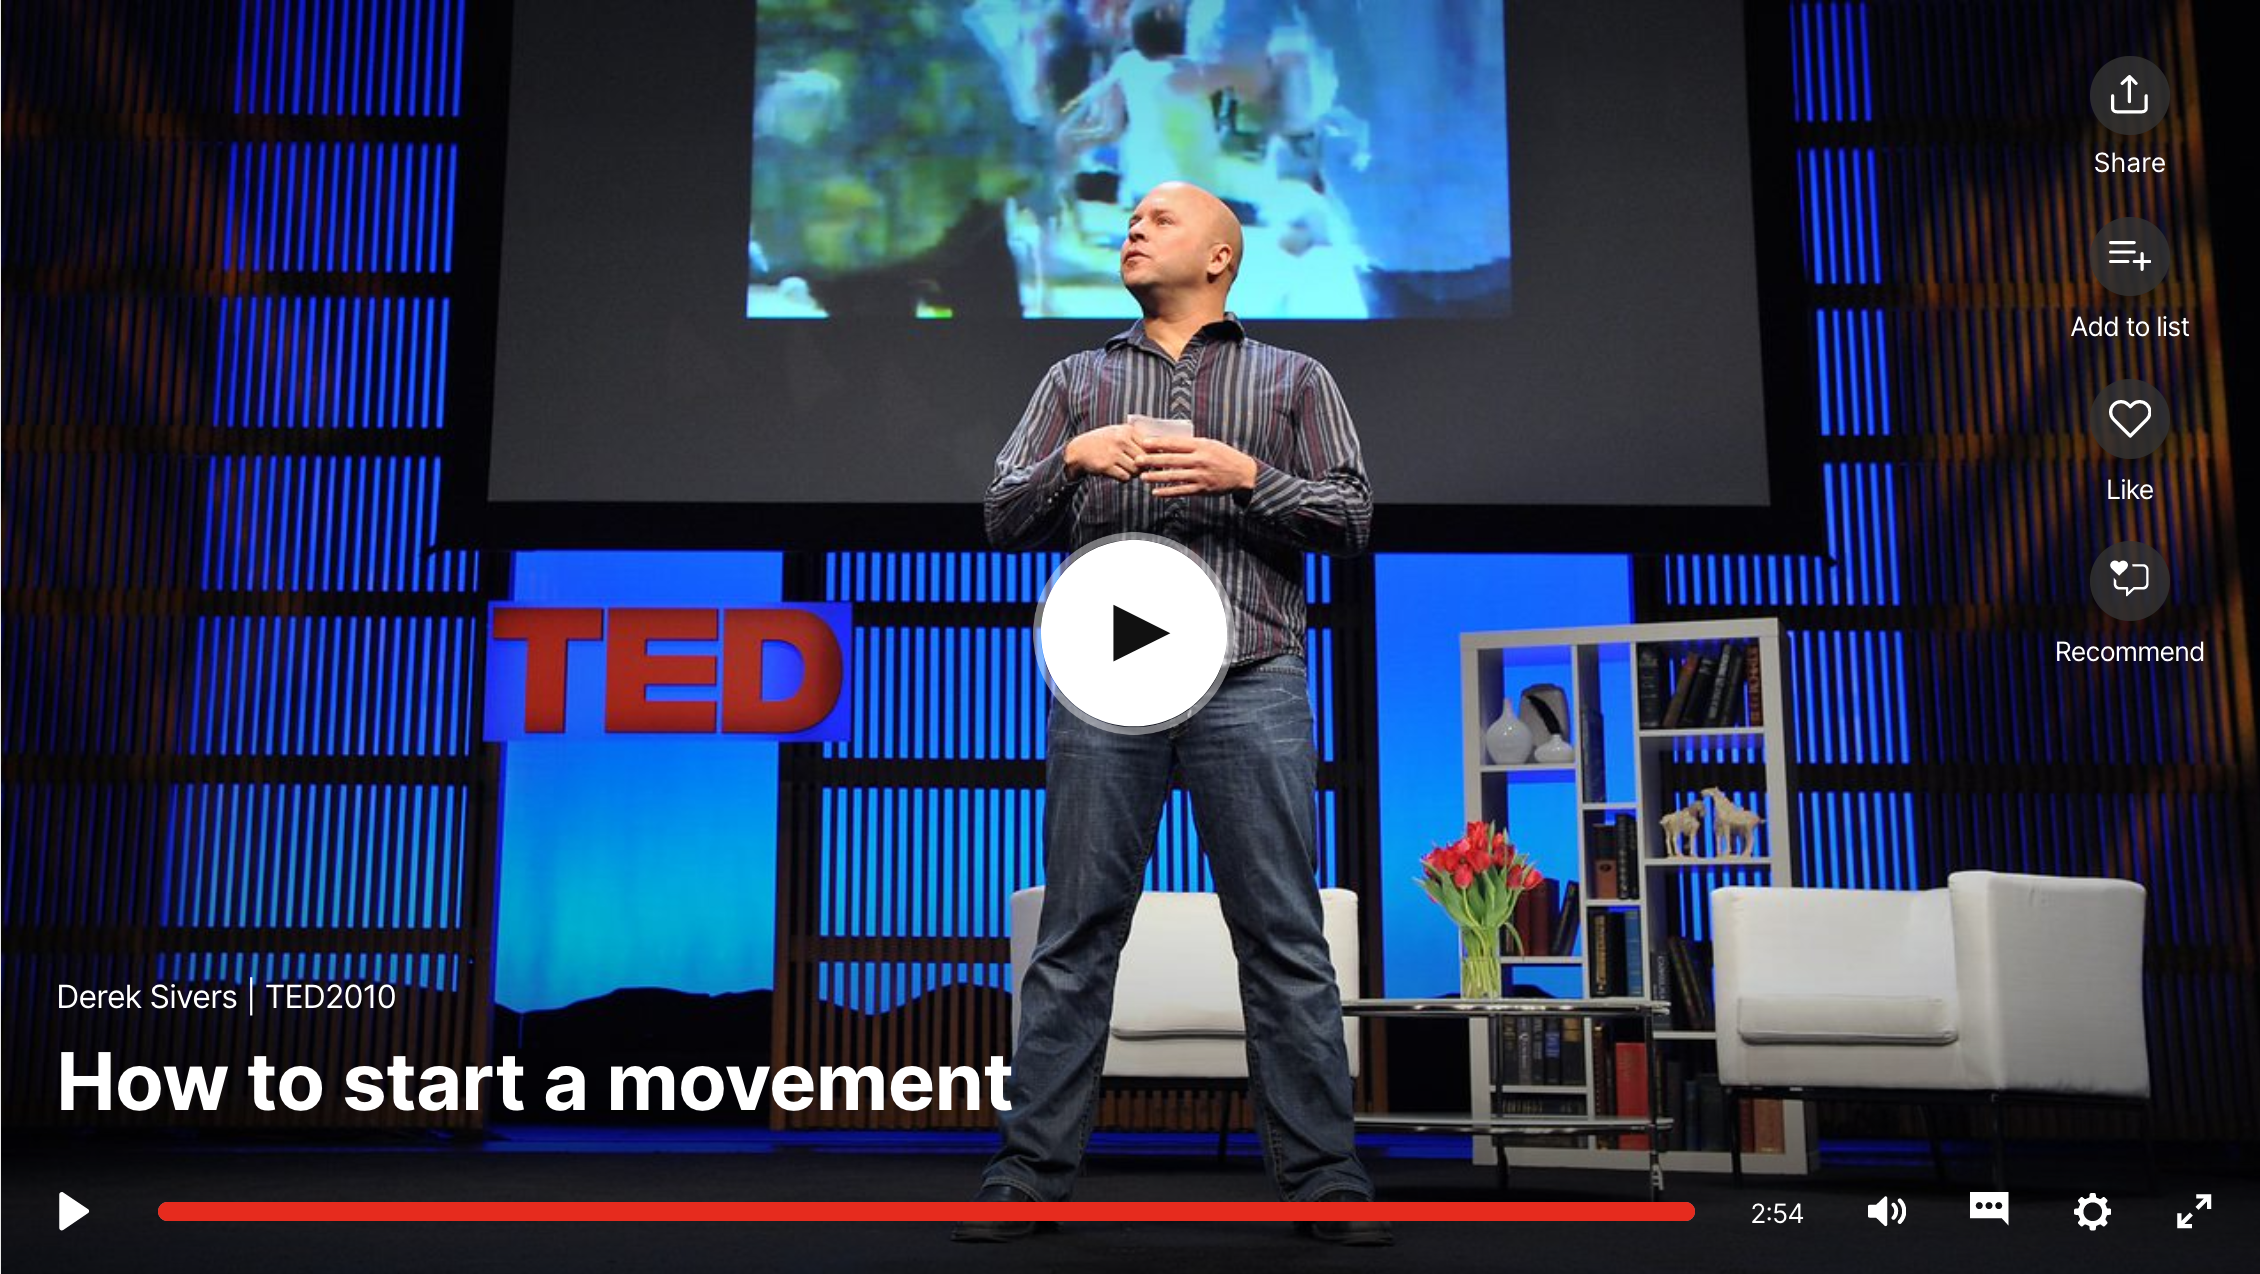
\includegraphics[width=0.8\textwidth]{figures/sivers_how_2010_title}
\end{center}

\vfill
\url{https://www.ted.com/talks/derek_sivers_how_to_start_a_movement\#t-169235}

\note{
Suggested by a former student
}

\end{frame}
%%%%%%%%%%%%%%%%%%%%%%%%%%%%
\begin{frame}

Now what happens if we move people using a threshold rule onto a network? 

\end{frame}


\end{document}
